% !TeX root = ./00.ppgcc-2020.tex

\begin{fichacatalografica}
   %     \includepdf{fig_ficha_catalografica.pdf}
   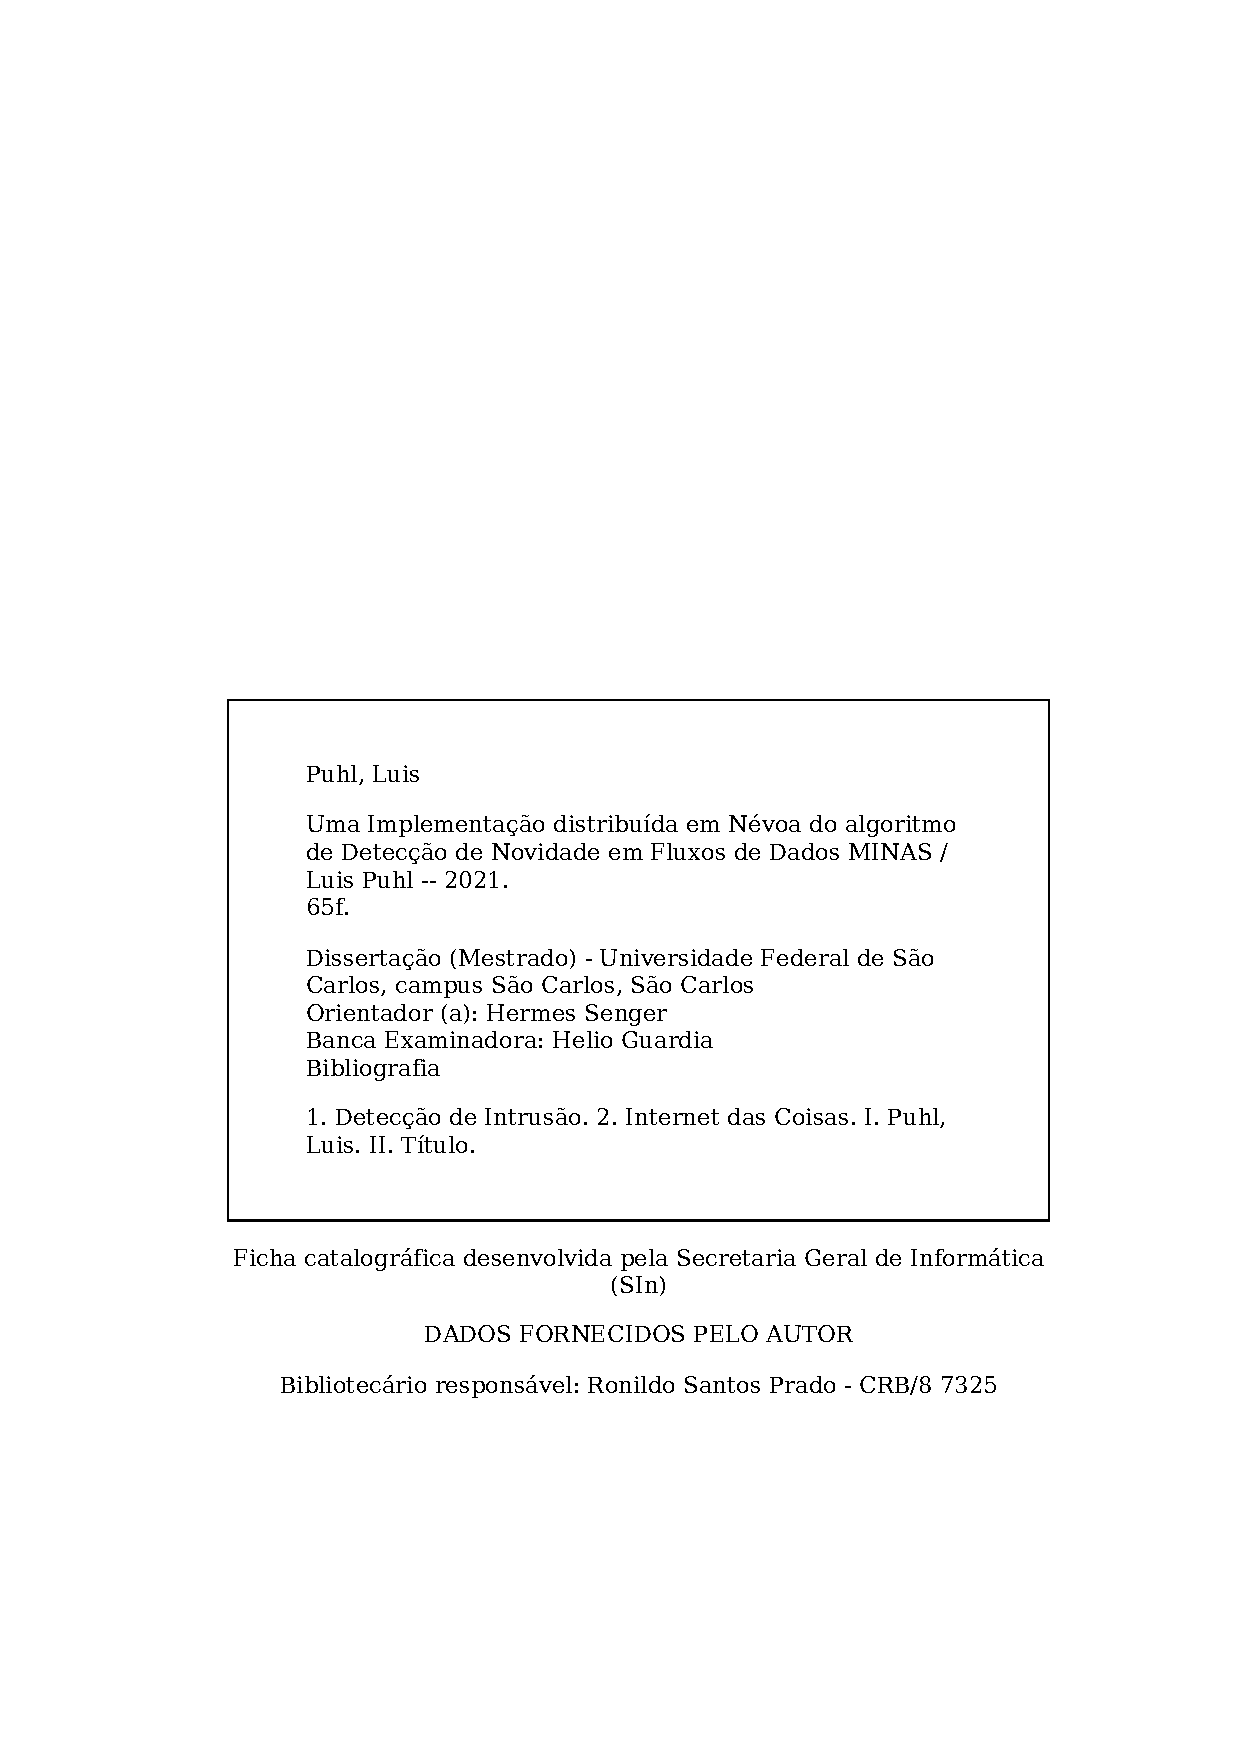
\includepdf{ficha-catalografica.pdf}
   % 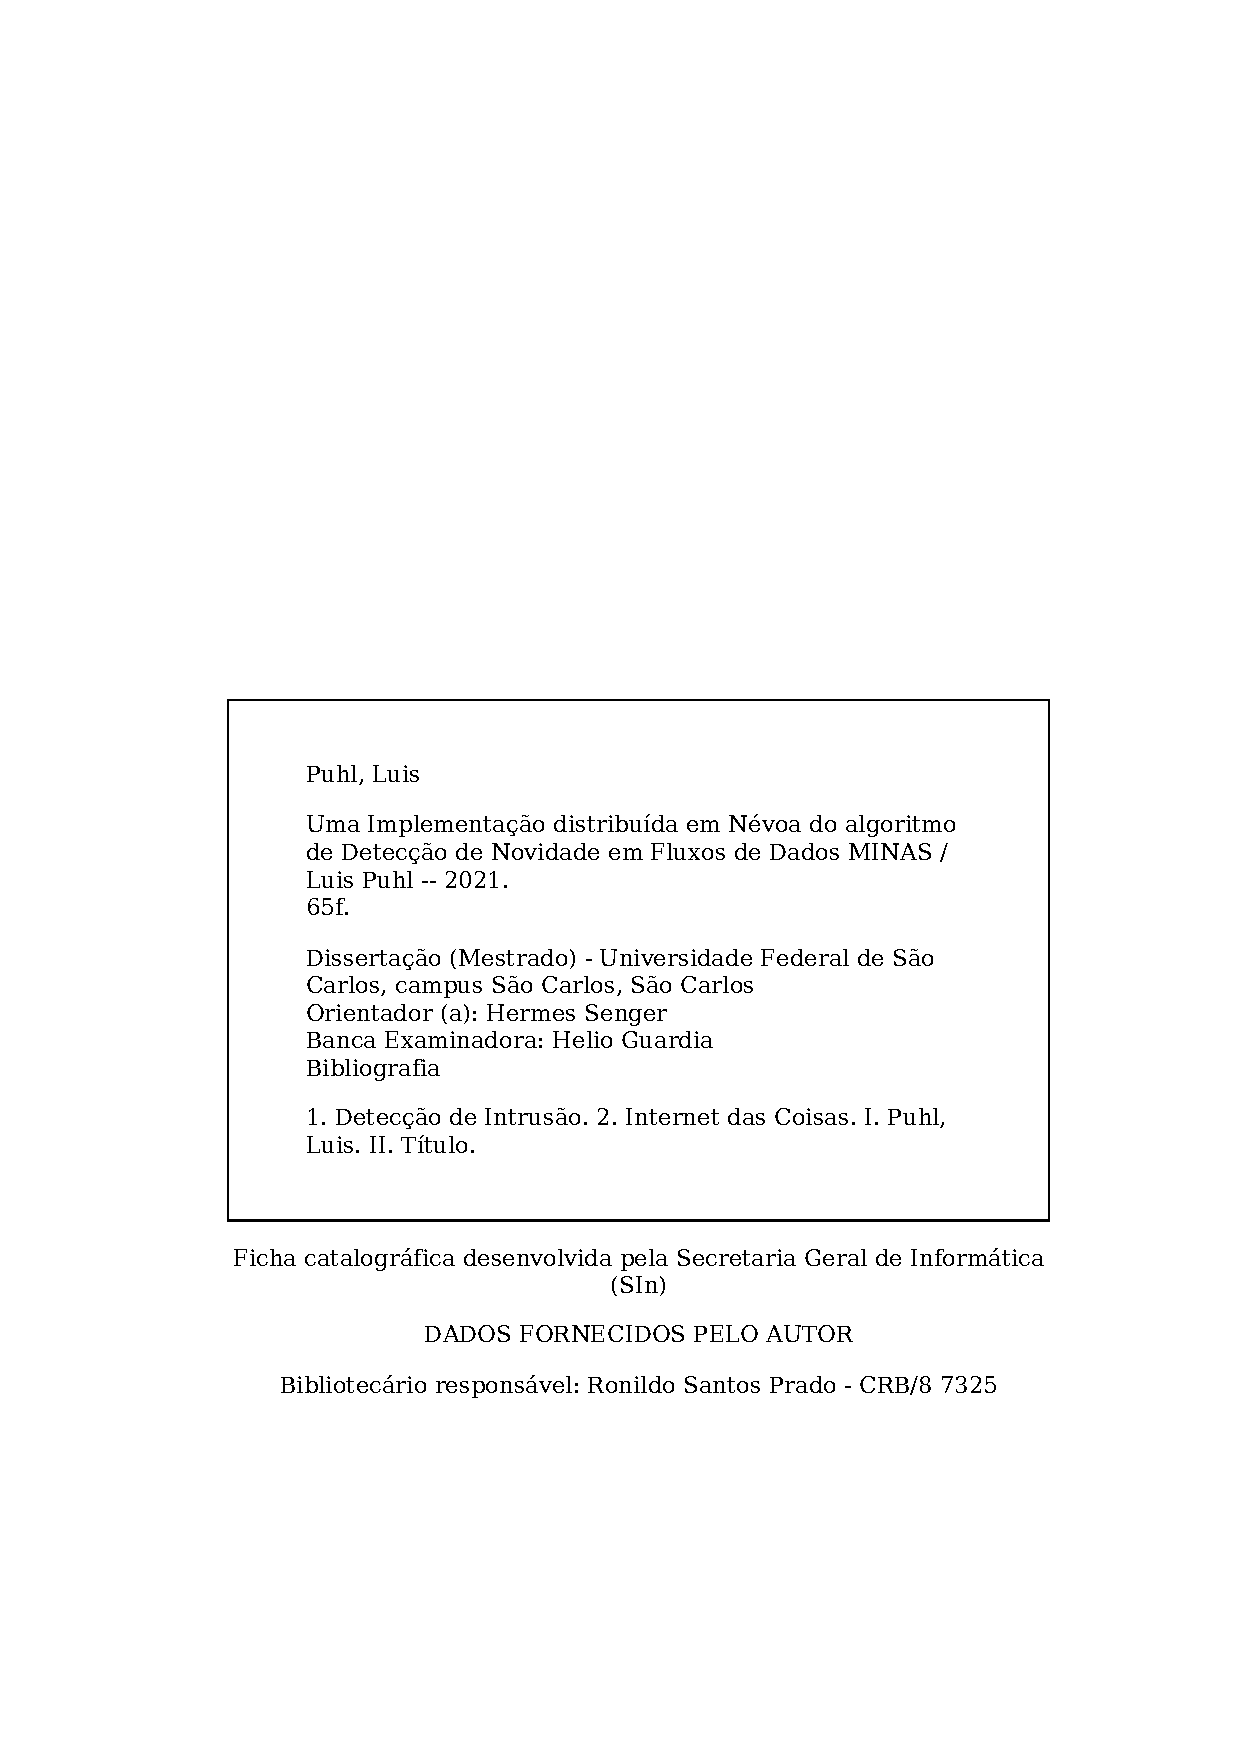
\includegraphics{ficha-catalografica.pdf}
   % \sffamily
   % \vspace*{\fill}                    % Posição vertical
   % \begin{center}                    % Minipage Centralizado
   %    \fbox{\begin{minipage}[c][8cm]{13.5cm}        % Largura
   %       \small
   %       % \imprimirautor
   %       % Puhl, Luís
   %       \authorbib
   %       %Sobrenome, Nome do autor
         
   %       \hspace{0.5cm} \imprimirtitulo  / \imprimirautor. --
   %       % \imprimirlocal, \imprimirdata-
         
   %       \hspace{0.5cm} \thelastpage{}f. : il. (algumas color.) ; 30 cm.\\
   %       % \pageref{LastPage}
         
   %       \hspace{0.5cm} \imprimirorientadorRotulo~\imprimirorientador\\
         
   %       \hspace{0.5cm}
   %       \parbox[t]{\textwidth}{\imprimirtipotrabalho~--~\@universidade
   %       % \imprimirinstituicao,
   %       \imprimirdata.}\\
         
   %       \hspace{0.5cm}
   %          1. Detecção de Intrusão.
   %          2. Internet das Coisas.
   %          I. Título.
   %          % I. Orientador.
   %          % II. Universidade Fede.
   %          % III. Faculdade de xxx.
   %          % IV. Título             
   %    \end{minipage}}
   % \end{center}
\end{fichacatalografica}

\begin{folhadeaprovacao}
   % \includepdf{folhadeaprovacao_final.pdf}
   %
   \noindent\begin{minipage}{0.3\textwidth}
      
\includegraphics[width=\linewidth]{lib/ufscar.pdf}
      \end{minipage}%
      \hfill%
      \begin{minipage}{0.7\textwidth}\center
      \imprimirinstituicao
   \end{minipage}
   % \begin{center}
   %    %   {\ABNTEXchapterfont\large\imprimirautor}

   %    %   \vspace*{\fill}\vspace*{\fill}
   %    %   \begin{center}
   %    %     \ABNTEXchapterfont\bfseries\Large\imprimirtitulo
   %    %   \end{center}
   %    %   \vspace*{\fill}

   %    %   \hspace{.45\textwidth}
   %    %   \begin{minipage}{.5\textwidth}
   %    %       \imprimirpreambulo
   %    %   \end{minipage}%
   %    %   \vspace*{\fill}
   % \end{center}
   
   \noindent\begin{minipage}{\textwidth}
      \begin{center}
      \rule{\linewidth}{1pt}
      % \vspace*{0.5ex}
      \textbf{Folha de Aprovação}\\[-0.5em]
      % \vspace*{-2ex}
      \rule{\linewidth}{1pt}
      % \hrule
      % \smash{\begin{tabular}{c} \hline  \\ \hline \end{tabular}\hspace*{-\tabcolsep}}
      % \frenchspacing
      % \hrulefill\\Folha de Aprovação\\\hrulefill
      \end{center}
   \end{minipage}

   % \vspace{2em}
   \begin{flushleft}
      Assinaturas dos membros da comissão examinadora que avaliou e aprovou a
      Defesa de Dissertação de Mestrado do candidato \imprimirautor{}, realizada
      % em \today{}:
      em 5 de Julho de 2021:
      %  Trabalho aprovado. \imprimirlocal, \today:
   \end{flushleft}
 
   % nome do Kelton fica mais longo que os 8cm padrão da classe abntex2
   % \setlength{\ABNTsignwidth}{10cm}
    \assinatura{\textbf{\imprimirorientador} \\ Presidente e Orientador}
   %  Hélio Crestana Guardia
   %  \assinatura{\textbf{Prof. Dr. Kelton Augusto Pontara da Costa} \\ Convidado}
   
    \assinatura{\textbf{Doutor Kelton Augusto Pontara da Costa} \\ Convidado}
   %  Paulo Matias
    \assinatura{\textbf{Doutor Paulo Sérgio Lopes de Souza} \\ Convidado}
   %  Júlio Cezar Estrella
    %\assinatura{\textbf{Professor} \\ Convidado 3}
    %\assinatura{\textbf{Professor} \\ Convidado 4}
       
   \vspace*{\fill}
   \begin{center}
      \vspace*{0.5cm}
      {\large\imprimirlocal}
      \par
      {\large\imprimirdata}
      \vspace*{1cm}
   \end{center}
\end{folhadeaprovacao}

% Dedicatória
% \imprimirdedicatoria{Este trabalho é dedicado às crianças adultas que,\\
%    quando pequenas, sonharam em se tornar cientistas.}
% Agradecimentos
\imprimiragradecimentos{
   % Carolina, Guilherme Cassales, Guilherme Raiol, Jaime, Lucian, Pedro,
   
   Agradeço os ensinamentos dos colegas, especialmente ao Professor Hélio,
   Professor Hermes e Doutor Guilherme pela experência compartilhada.
   
   Agradeço à companheira Carolina pela constante alegria e apoio a todos os
   momentos e ao incentivo e ajuda nas horas difíceis.

   Agradeço aos familiares e amigos pelo carinho.
   
   Agradeço também ao CNPq pelo suporte %\hlke{financiero} 
   financeiro (contrato 167345/2018-4).
}
% Epígrafe
% \imprimirepigrafe{
%         ``Somos essencialmente profissionais do sentido. Educamos, \\
%          quando ensinamos com sentido. Educar é impregnar de sentido\\
%          a vida. A profissão docente está centrada na vida, no bem querer.''\\
%         (Prof. Gilberto Teixeira)
% }

% RESUMO e ABSTRACT
\begin{resumo}{Detecção de Novidades. Detecção de Intrusão. Fluxos de Dados.
   Computação Distribuída. Computação em Névoa. Internet das Coisas}

   % \notaPA{FALAR NO FINAL DA ARGUIÇÃO:
   % 
   % O trabalho não encontrou eficiência no uso da versão distribuída/paralela,
   % característica chave
   % para a eficácia na detecção de intrusão. Sugiro mudar o objetivo de propor um
   % sistema ... para avaliar o uso da computação distribuída, levantando
   % virtudes, desafios e requisitos.
   % 
   % Isso já está na introdução, página 15.
   % }

   Em um cenário de crescente número de dispositivos na Internet das Coisas
   (IoT), gerando um crescimento %\hlpa{proporcional}
   no volume dos fluxos de dados
   gerados,
   % são necessários métodos robustos para a mineração de fluxos contínuos de dados.
   são constantes e evolutivas as ameaças ativas e passivas aos recursos
   computacionais e aos conteúdos transmitidos.
   % 
   Métodos para mineração de dados de forma robusta e contínua podem ser um
   aliado à segurança nesses casos.
   % 
   % \hlke{a onde eles}
   Particularmente em ambientes distribuídos e nos quais busca-se manter o tratamento
   dos fluxos de informação próximo de onde eles são gerados, como nas bordas das
   redes IoT, e na computação em névoa de maneira geral, a detecção de ameaças é
   essencial e não trivial.
   % 
   % Uma das áreas afetadas pelo crescimento vertiginoso do número de
   % dispositivos e os fluxos associados a eles é a área de segurança da
   % informação, onde são necessárias ferramentas de detecção de intrusão em redes
   % que operem em ambientes de computação em névoa, devido aos custos de
   % comunicação associados a operar estas ferramentas somente em ambiente de
   % nuvem.
   Além disso, a evolução constante dos tipos de dispositivos e de tráfegos
   nessas redes favorece que as ferramentas de detecção de ameaças sejam
   beneficiadas por algoritmos de Detecção de Novidades em Fluxo de Dados.
   % beneficiadas por \hlpa{algoritmos de Detecção de Novidades em Fluxo de Dados}.
   % \notaPA{Tricorder?}
   % 
   % % As ferramentas de detecção de intrusão utilizam extensivamente algoritmos
   % % de detecção de novidade em fluxos de dados para identificar padrões no
   % % tráfego da rede.
   % % Porém, os algoritmos que tratam adequadamente dos desafios de detecção de
   % % novidade em fluxos de dados, como mudança e evolução de conceito e
   % % atualização contínua do modelo de classificação sem interferência de
   % % especialistas, ainda são pouco utilizados.
   % 
   MINAS é um exemplo de algoritmo de detecção de novidades em fluxos de dados
   com potencial para aplicação na computação em névoa.
   %
   % % O algoritmo de detecção de novidade em fluxo de dados MINAS tem recebido
   % % atenção de pesquisas recentes por tratar desses desafios de detecção de
   % % novidade em fluxos de dados.
   % 
   No entanto,
   %\hlpa{
   apesar de sua divisão em três partes semi-independentes, este
   algoritmo ainda não foi adaptado para tratar grandes volumes de fluxos
   reais em ambiente de computação em névoa.
   % }
   % \notaPA{A versão distribuída está adaptada, porém, não é eficiente, impedindo
   % a eficácia daquilo que se propõe.}
   % 
   O presente trabalho aborda essa lacuna propondo um sistema que implementa o
   algoritmo MINAS de maneira distribuída inserido num contexto
   de detecção de intrusão e computação em névoa.
   % 
   Esta implementação foi feita em MPI e é avaliada com auxílio do conjunto de
   dados \emph{Kyoto 2006+} em um ambiente de teste com 3 nós com recursos
   limitados.
   Os resultados obtidos mostram a viabilidade do modelo de detecção de
   novidades distribuído em ambiente de computação em névoa.
   % 
   Observou-se baixa degradação nas métricas de classificação porém com redução
   no número de novidades (anomalias, ataques) encontradas.
   Além disso, observou-se redução do tempo de processamento na nova
   implementação distribuída em relação à implementação original, porém o
   \emph{speedup} não refletiu a adição de processadores.
   % na execução paralela e distribuída indic abaixo do esperado.
   
   % \textcolor{red}{TODO: Revisar este fechamento, não agradou ao Paulo.}\\
   % \notaPA{
   % Por que ``Mesmo'' em um cenário distribuído? Qual a dificuldade pelo fato de 
   % ser distribuído.
   % }
   % ``No entanto''? Quero dizer que mesmo com 12 CPUs não obteve resultado melhor.
   % \hlpa{Mesmo em um cenário distribuído}, 
   % \hlpa{o sistema apresentou eficácia equivalente ao}
   % \notaPA{
   % O problema a ser resolvido era que o algoritmo ainda não havia sido adaptado
   % para processar grandes volumes de fluxos reais em computação em névoa. Mas o
   % algoritmo original funcionava para computação em névoa para suportar esta
   % afirmação?
   % % O MINAS não é adaptado para névoa, tanto no sentido distribuído quanto uso
   % % de recursos.
   % % Author: O original foi testado em névoa por Cassales2019
   % }
   % algoritmo original, ainda que executando em dispositivos de capacidade
   % computacional limitada, como é previsto em cenários de IoT.

\end{resumo}

% Resumo em inglês
\begin{abstract}{Novelty Detection. Intrusion Detection. Data Streams.
   Distributed Computing. Fog Computing. IoT devices}

   % In a scenario of growing number of devices connected to the Internet of Things (IoT)
   % with proportional growth in the volume of data streams generated, robust
   % methods are needed for mining streams continuous data.
   % %%
   % One of the areas affected by the huge growth in the number of devices
   % and the streams associated with them is the information security, which needs
   % network intrusion detection tools that operate
   % in fog computing environments due to the cost of operating such tools
   % in a cloud only environment.
   % %%
   % These tools make extensive use of algorithms for novelty detection in data
   % streams to identify treat patterns in network traffic.
   % However, algorithms in wide use do not
   % adequately address the challenges of novelty detection in data streams,
   % such as concept drift, concept evolution and continuous update of the
   % classification model, without expert interference.
   % %%
   % The MINAS algorithm addresses those novelty detection in data streams
   % challenges and has received recent research attention.
   % %%
   % However, despite its division in three semi-independent parts, MINAS has
   % not yet been adapted to process large volumes of real streams or to operate
   % in a fog computing environment.
   % %%
   % The present work proposes a system that implements the MINAS algorithm
   % in a distributed fog environment in the context of intrusion detection
   % to addresses this gap.
   % %%
   % Preliminary work shows that it is possible to have a distributed
   % version of the MINAS algori thm by using stream processing platforms
   % such as Apache Flink.

   The ongoing implementation of the Internet of Things (IoT) is sharply
   increasing the number and variety of small devices on edge networks.
   %
   Likewise, the attack opportunities for hostile agents also
   % increase\hlke{s}, requiring more effort from network administrators and strategies
   grows, requiring more effort from network administrators and strategies
   to detect and react to those threats.
   % 
   For a network security system to operate in the context of fog and
   IoT, it has to comply with processing, storage, and energy
   requirements alongside traditional requirements for stream and network
   analysis like accuracy and scalability.
   % 
   Using a previously defined architecture (IDSA-IoT), we address the construction
   and evaluation of a support mechanism for distributed Network Intrusion
   Detection Systems (NIDS) based on the MINAS Data Stream Novelty Detection
   % (DSND)
   algorithm.
   % 
   We discuss the algorithm steps, how it can be deployed in a distributed
   % environment, the impacts on the accuracy\hlke{,} and evaluate performance and
   environment, the impacts on the accuracy, and evaluate performance and
   scalability using a cluster of constrained devices commonly found in IoT
   scenarios.
   % 
   The obtained results show equivalent metrics in the distributed version but
   % also a reduction in the execution time using \hlke{low-profile} devices.
   also a reduction in the execution time using low-profile devices.
   Although not efficient, the parallel version showed to be viable as the
   % proposed granularity provides equivalent accuracy and \hlke{the} same response times.
   proposed granularity provides equivalent accuracy and the same response times.
   % \todo[inline]{Poderia dizer que não houve redução do tempo de execução. }

\end{abstract}
